\documentclass[12pt]{article}
\usepackage{amsmath}
\usepackage[unicode=true, colorlinks=true, linkcolor=blue, urlcolor=cyan]{hyperref}
\usepackage{graphicx}
\usepackage{float}
\usepackage{caption}
\usepackage{listings}
\usepackage{xcolor} 
\usepackage{pgfplots}
\usepackage{tikz}
\usetikzlibrary{snakes}
\usepackage{rotating}
\usetikzlibrary{arrows.meta, shapes}
\usepackage{pdflscape}   % Landscape pages
\usepackage[backend=biber,style=alphabetic]{biblatex} % Bibliography management
\addbibresource{references.bib} % Bibliography file
\graphicspath{{doc/}}


% Define colors
\colorlet{punct}{red!60!black}
\definecolor{background}{RGB}{240, 248, 255} % Pale Blue
\definecolor{delim}{RGB}{20,105,176}
\colorlet{numb}{magenta!60!black}

% Define JSON language
\lstdefinelanguage{json}{
    basicstyle=\ttfamily\footnotesize\color{black},
    basicstyle=\ttfamily\footnotesize\color{black},
    numbers=left,
    numberstyle=\scriptsize,
    stepnumber=1,
    numbersep=8pt,
    showstringspaces=false,
    breaklines=true,
    frame=lines,
    backgroundcolor=\color{background},
    literate=
     *{0}{{{\color{numb}0}}}{1}
      {1}{{{\color{numb}1}}}{1}
      {2}{{{\color{numb}2}}}{1}
      {3}{{{\color{numb}3}}}{1}
      {4}{{{\color{numb}4}}}{1}
      {5}{{{\color{numb}5}}}{1}
      {6}{{{\color{numb}6}}}{1}
      {7}{{{\color{numb}7}}}{1}
      {8}{{{\color{numb}8}}}{1}
      {9}{{{\color{numb}9}}}{1}
      {:}{{{\color{punct}{:}}}}{1}
      {,}{{{\color{punct}{,}}}}{1}
      {\{}{{{\color{delim}{\{}}}}{1}
      {\}}{{{\color{delim}{\}}}}}{1}
      {[}{{{\color{delim}{[}}}}{1}
      {]}{{{\color{delim}{]}}}}{1},
}



\setlength{\parskip}{1em}

\lstset{frame=single, showstringspaces=false, columns=fixed, basicstyle={\ttfamily}, commentstyle={\it}, numbers=left, tabsize=4}

\definecolor{codebackground}{RGB}{240, 248, 255}
\definecolor{codecomment}{RGB}{106,153,85}
\definecolor{codekeyword}{RGB}{30,30,255}
\definecolor{codestring}{RGB}{163,21,21}
\definecolor{codenumber}{RGB}{100,100,100}

\lstdefinestyle{modernstyle}{
    backgroundcolor=\color{codebackground},
    commentstyle=\color{codecomment},
    keywordstyle=\color{codekeyword},
    numberstyle=\tiny\color{codenumber},
    stringstyle=\color{codestring},
    basicstyle=\ttfamily\footnotesize\color{black},
    breakatwhitespace=false,
    breaklines=true,
    captionpos=b,
    keepspaces=true,
    numbers=left,
    numbersep=5pt,
    showspaces=false,
    showstringspaces=false,
    showtabs=false,
    tabsize=4
}


\lstset{style=modernstyle}

\begin{document}

\begin{titlepage}
\centering

\includegraphics[width=0.5\textwidth]{images/logo-ufr.png}\par\vspace{1cm}
\vspace{1.5cm}
{\huge\bfseries M2-Project: \\
Pre and Post-Processing applied to a LNCMI Bitter Magnet\par}
\vspace{2cm}
{\Large Pierre-Antoine Senger and Antoine Regardin\par}
\vfill


\vfill

% Bottom of the page
{\large Date: \today\par}
\end{titlepage}

\tableofcontents

\newpage

\section{Introduction}

\subsection{Context}
A Bitter magnet is a type of electromagnet that uses stacked, flat, spiral-shaped 
copper or brass plates (discs) with slits to allow cooling water to flow through. 
Due to their ability to handle large electric currents without overheating and
generating strong magnetic fields, Bitter electromagnets are widely used in
high-field physics research, such as nuclear magnetic resonance (NMR) and magnetic
resonance imaging (MRI) machines.

Simulations of how current and heat are distributed in the magnet are crucial to
understand the behavior of the magnet to maximize its performance and prevent
overheating and irreversible damages.

\begin{figure}[H]
	\centering
	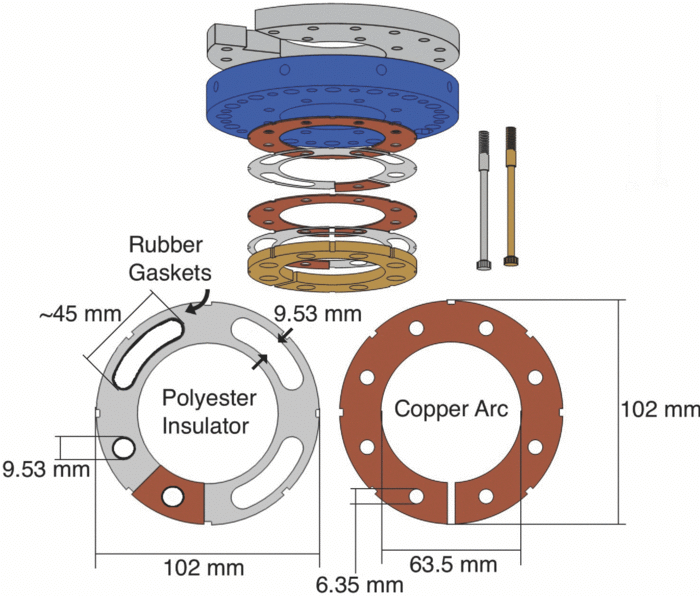
\includegraphics[width=0.8\textwidth]{images/Bitter-electromagnet-breakout.png}
	\caption{Breakout of a Bitter electromagnet \cite{bitter_breakout}}
\end{figure}

\subsection{Main objectives}

\begin{itemize}
	\item Model the Bitter magnet geometry and mesh it with an adaptive mesh.
	\item Run simulations to study the distribution of current and heat in the magnet.
	\item Visualize the results and analyze the behavior of the magnet.
\end{itemize}

\subsection{Software and libraries}
To make the model of the Bitter and mesh it, we will use Gmsh \cite{geuzaine_gmsh_2009}, a three-dimensional
 finite element mesh generator with a built-in CAD engine and post-processor. 
Gmsh is an open-source software and is widely used in the scientific
community.

As for our simulations, our primary tool will be Feel++\cite{christophe_prudhomme_feelppfeelpp_2024}, a robust and 
efficient open-source C++ library designed for solving partial differential equations using 
the finite element method\cite{fem}.



\section{Methodology}
\subsection{Geometry and mesh generation}

\begin{figure}[H]
	\centering
	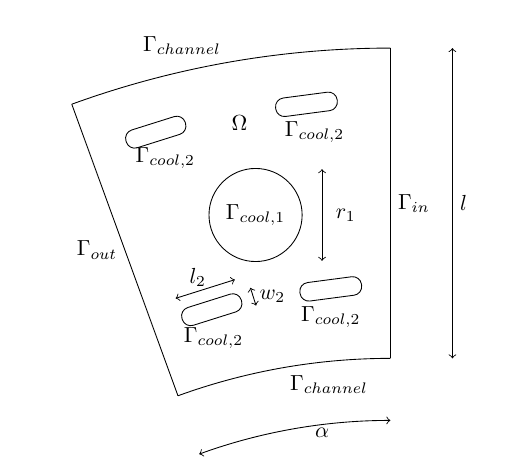
\includegraphics[width=0.8\textwidth]{images/top_view_bitter.png}
	\caption{Top view of the geometry of the LNCMI Bitter magnet.}
\end{figure}

\begin{table}[H]
	\centering
	\begin{tabular}{|l|c|c|c|}
	\hline
	\textbf{Parameter} & \textbf{Symbol} & \textbf{Units} & \textbf{Value} \\ \hline
	Internal radius & $r_i$ & mm & 200 \\ \hline
	Length of the bitter & $l$ & mm & 100 \\ \hline
	Angle between $\Gamma_\text{in}$ and $\Gamma_\text{out}$ & $\alpha$ & radian & $\pi/18$ \\ \hline
	Diameter of $\Gamma_\text{cool,1}$ & $r_1$ & mm & 10 \\ \hline
	Width of $\Gamma_\text{cool,2}$ & $w_2$ & mm & 1.1 \\ \hline
	Length of $\Gamma_\text{cool,2}$ & $l_2$ & mm & 5.9 \\ \hline
	Height & - & mm & 4 \\ \hline
	\end{tabular}
	\caption{Geometrical parameters for the Bitter magnet.}
	\label{tab:bitter_geometry}
	\end{table}

To correctly places the points of the mesh at the right position we converted polar
coordinates to cartesian coordinates using the relations:
$$
\begin{cases}
	x = \rho \cos(\theta) \\
	y = \rho \sin(\theta)
\end{cases}
$$

Physical groups were defined for each boundary of the geometry to apply the boundary conditions.

\begin{figure}[H]
	\centering
	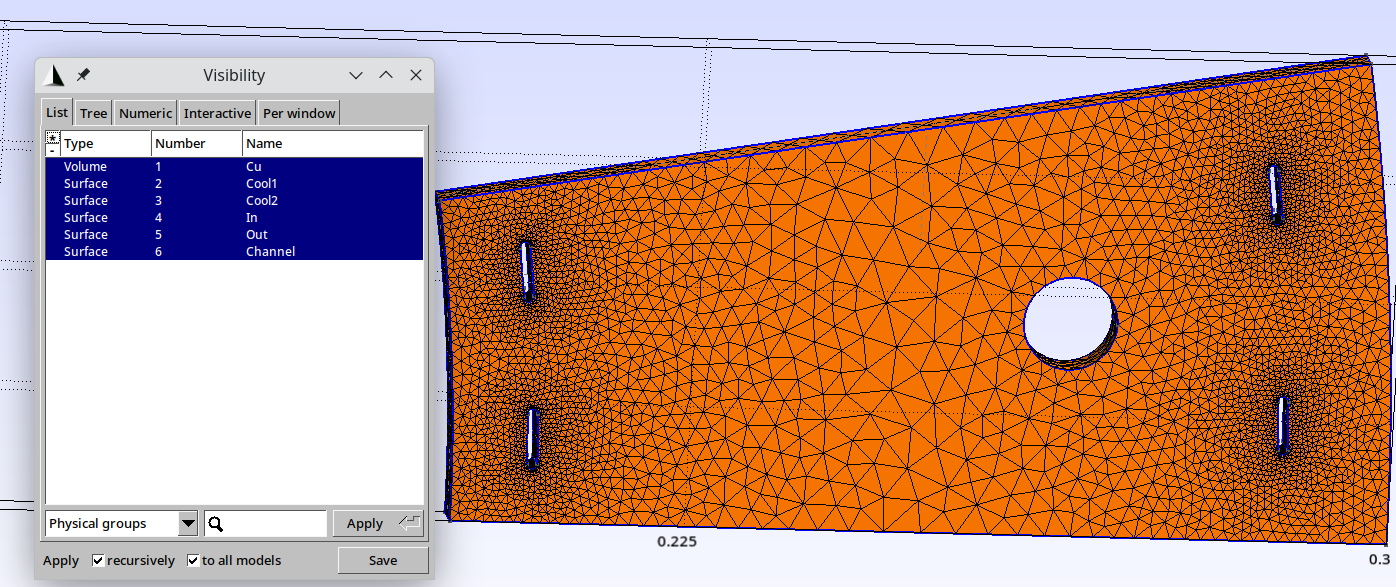
\includegraphics[width=\textwidth]{images/bitter_mesh.png}
	\caption{Adaptive 3D mesh of the LNCMI Bitter magnet.}
\end{figure}

\subsection{Mathematical model}
The heat is modeled using the heat equation:
$$
	-\nabla \cdot (\kappa \nabla T) = 0 \quad \text{in } \Omega 
$$
Where $\kappa$ is the thermal conductivity of the material.

\noindent And we used the following Poisson equation for electric potential:
$$
	\nabla^2 V = -\frac{I}{\sigma} \quad \text{in } \Omega
$$
Where $I$ is the current intensity and $\sigma$ is the electric conductivity of the material.  

To close the system, we used the following boundary conditions:

\begin{table}[H]
	\centering
	\begin{tabular}{|l|l|l|}
	\hline
	\textbf{Name} & \textbf{Heat} & \textbf{Electric} \\ \hline
	In & Neumann homogeneous & Dirichlet $V = 0$ \\ \hline
	Out & Neumann homogeneous & Dirichlet $V = 0.03125$ \\ \hline
	Channel & Robin ($h_e$, $T_{w,e}$) & - \\ \hline
	Cool1 & Neumann homogeneous & - \\ \hline
	Cool2 & Robin ($h_i$, $T_{w,i}$) & - \\ \hline
	\end{tabular}
	\caption{Boundary conditions.}
	\label{tab:boundary_conditions}
\end{table}

Both models were discretized using the finite element method (variational formulation).

\subsection{Simulation}
\begin{minipage}[t]{0.49\textwidth}
\raggedright
The simulations were performed on the High-Performance Computing (HPC) cluster Gaya. 
This cluster consists of a DELL PowerEdge R7525 head node and six DELL PowerEdge 
R6525 compute nodes, providing a total of 768 multi-threaded cores on the compute 
nodes and 96 cores on the head node. Gaya offers 150 TB of storage for data and 
an extremely fast 15 TB NVME scratch space. The head node is equipped with two AMD EPYC 7552 48-Core Processors running at 
2.2GHz, totaling 192 virtual cores, and 1024 GB of RAM. 
\end{minipage}
\hfill
\begin{minipage}[t]{0.49\textwidth}
\raggedleft
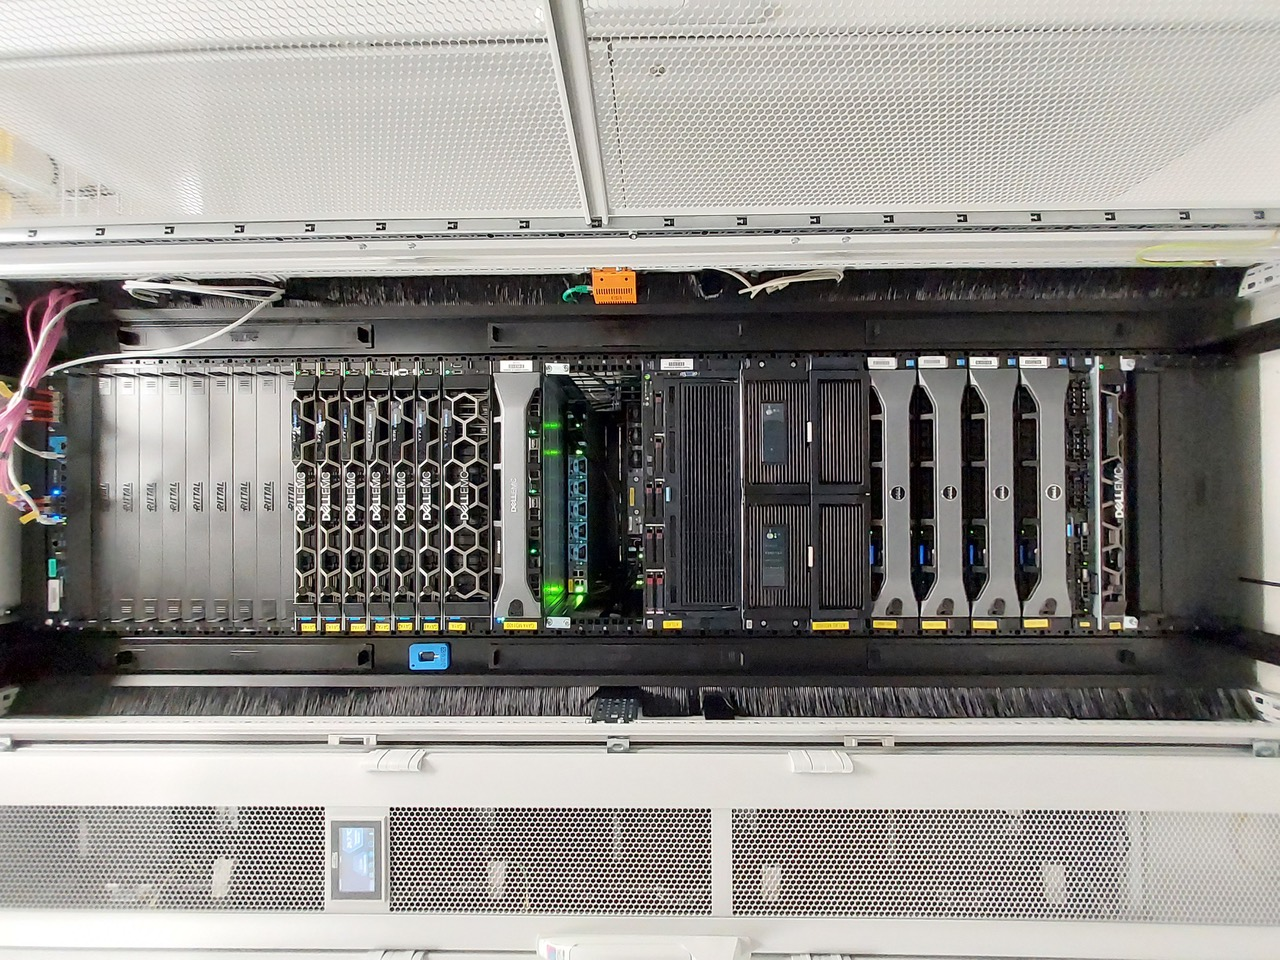
\includegraphics[width=1.1\textwidth, angle=-90]{images/gaya.jpeg}
\captionof{figure}{Gaya supercomputer.}
\end{minipage}

\noindent Each compute node features two AMD EPYC 7713 64-Core Processors running at 2GHz, 
totaling 256 virtual cores, and 512 GB of RAM. The nodes are interconnected via 
Broadcom Adv. Dual 10GBASE-T Ethernet and Mellanox ConnectX-6 Dx Dual Port 100 
GbE for MPI communication.

We used the following input parameters and physical properties:

\begin{table}[H]
	\centering
	\begin{tabular}{|l|l|c|c|}
	\hline
	\textbf{Name} & \textbf{Description} & \textbf{Value} & \textbf{Unit} \\ \hline
	$I$ & Current intensity & $-800$ & A \\ \hline
	$V_D$ & Electrical potential & $0.03125$ & V \\ \hline
	$h_i$ & Internal transfer coefficient & $0.08$ & $\mathrm{W \cdot mm^{-2} \cdot K^{-1}}$ \\ \hline
	$T_{w,i}$ & Internal water temperature & $293$ & K \\ \hline
	$h_e$ & External transfer coefficient & $0.08$ & $\mathrm{W \cdot mm^{-2} \cdot K^{-1}}$ \\ \hline
	$T_{w,e}$ & External water temperature & $293$ & K \\ \hline
	\end{tabular}
	\caption{Input parameters.}
	\label{tab:input_parameters}
	\end{table}

	\begin{table}[H]
		\centering
		\begin{tabular}{|l|l|c|c|c|}
		\hline
		\textbf{Name} & \textbf{Description} & \textbf{Marker} & \textbf{Value} & \textbf{Unit} \\ \hline
		$\sigma$ & Electric conductivity & omega & $58 \cdot 10^3$ & $\mathrm{S \cdot mm^{-1}}$ \\ \hline
		$\kappa$ & Thermal conductivity & omega & $0.38$ & $\mathrm{W/(mm \cdot K)}$ \\ \hline
		\end{tabular}
		\caption{Physical properties (Cu).}
		\label{tab:physical_properties}
	\end{table}


			

\section{Implementation}


\section{Results Visualization}
\begin{figure}[H]
	\centering
	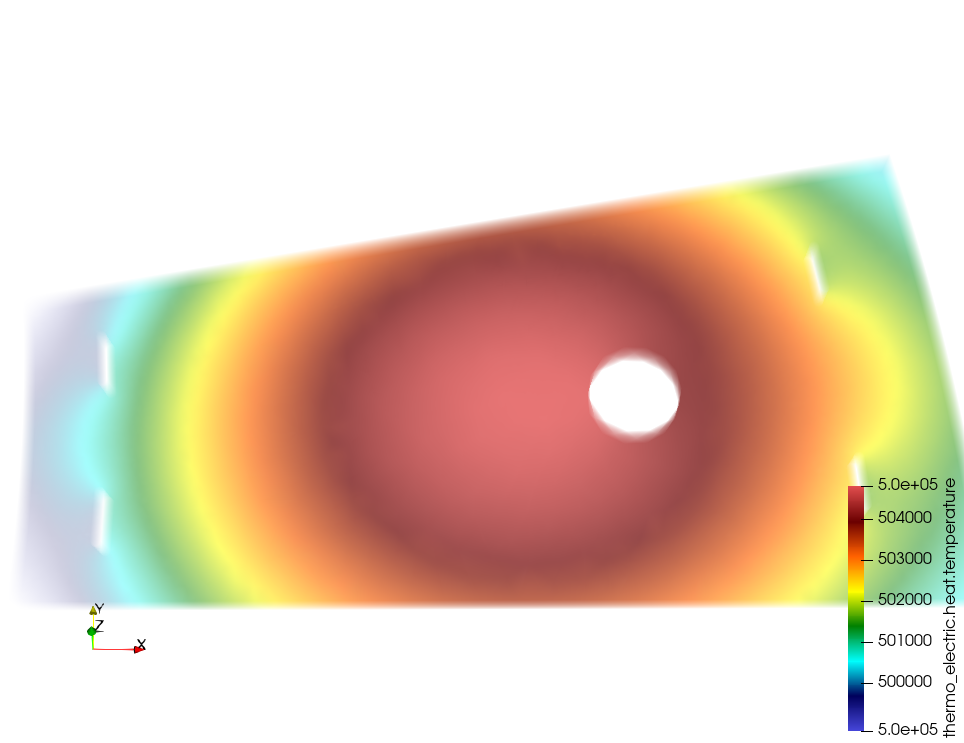
\includegraphics[width=0.8\textwidth]{images/heat.png}
	\caption{Heat distribution in the Bitter magnet.}
\end{figure}
\begin{figure}[H]
	\centering
	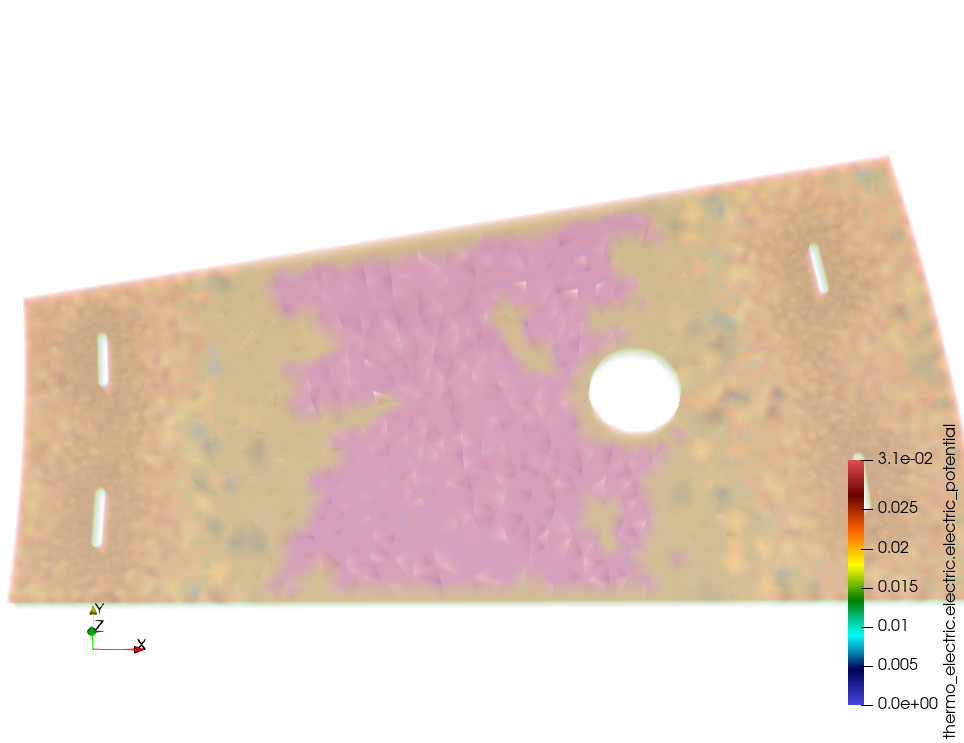
\includegraphics[width=0.8\textwidth]{images/electric_potential.png}
	\caption{Electric potential distribution in the Bitter magnet.}
\end{figure}


\section{Prospects}
\begin{enumerate}
	\item Improve mesh slits generation by making a function to generate them.
	\item Make the mesh parametrizable to change the geometry of the Bitter magnet 
	(e.g., radius, length, number of slits, etc.).
	\item Test the model with different materials, physical properties, boundary conditions, etc.
	\item Make a complexity analysis of the simulation depending on the number of elements of the mesh.
\end{enumerate}

\section{Conclusion}

\newpage

\section{References}
\printbibliography
\end{document}